\chapter{Opdracht}
In dit hoofdstuk wordt beschreven bij welke organisatie de opdracht zich afspeelt. Wat waren de ontwikkelingen binnen de organisatie en wat zijn de redenen om een nieuw project te starten?

\section{Achtergrond}

Shop2market is een software development bedrijf in de business-to-business sector. Het bedrijft heeft een missie om organisaties te helpen de winst uit online advertentiecampagnes te maximaliseren. 
Voor alsnog diende Shop2market
%, een integratie tool voor bijna alles betreft advertentie management,
als een IT oplossing ondersteunend aan het adviesbedrijf. Een grootte hoeveelheid van deze klanten waren webwinkels in het A segment. Maar omdat de integratie met een webwinkel vaak maatwerk opleverde, duurde een integratie gemiddeld zes tot acht maanden. Hieruit valt ook te concluderen dat veel bedrijven niet de technologische middelen in huis hebben om zelfstandig te kunnen starten met adverteren.

Daarom werd in begin 2015 gestart met de ontwikkeling van een nieuwe dienst: Adcurve. Met alle ervaring vanuit de adviesorganisatie zijn veel processen vertaald naar functionaliteiten. Door de diverse functionaliteiten\footnote{ Denk hierbij aan datavisualiasties en beheeracties, soms ook wel "Actionable insights"\  genoemd.} in Adcurve kan de webwinkeleigenaar zijn online marketing campagnes controleren en binnen budget houden. Dit is mogelijk doordat Adcurve een partij is tussen de webwinkel en publishers. Door platform zoals SEOShop of Magento is het mogelijk webwinkels binnen enkele minuten te integreren. 
Op basis van verzamelde gegevens zoals afkomstige bezoeken, bestellingen en advertentiekosten worden de nodige statistieken berekend. Met deze gegevens wordt de winstgevendheid per advertentie berekend.


Dit alles heeft als gevolg dat Shop2market op dit moment webwinkels in het midden en klein bedrijf  bedient, maar internationaal op een veel groter volume. Webwinkels zijn nu binnen enkele minuten geïnstalleerd en kunnen hun producten gemakkelijk adverteren via zogeheten publishers. Publishers zijn de bedrijven die de advertenties publiceren. Het soort advertenties verschillen nogal per publisher. Denk bijvoorbeeld aan ingekochte zoekresultaten, producten op prijsvergelijkers of affiliaties, maar ook producten op marktplaatsen. De gebruiker kan zelf publishers installeren binnen Adcurve zodat de benodigde integratie automatisch wordt afgehandeld. 

\clearpage

\section{Aanleiding} % de aanleiding tot de opdracht

De afgelopen maanden zijn er vijf publishers geïntegreerd waarvoor een volledige data integratie is ontwikkeld. Bij deze publishers worden kosten niet door ons berekend op basis van een percentage of vast bedrag. De kosten die in rekening zijn gebracht worden gerapporteerd en door Adcurve geïmporteerd.
Omdat de belangrijkste functionaliteiten berusten op de beschikbaarheid van statistiek gegevens ligt dit proces aan de kern van de dienst. Het verwerken van de data bronnen verloopt niet altijd zonder fouten. Door de gewenste groei is het een prioriteit geworden om de datakwaliteit te kunnen waarborgen. In de huidige situatie is het nog lastig om te herstellen van fouten, doordat het berekenen van de statistieken een langzaam proces is.

Er is hierdoor een toenemende wens ontstaan om de huidige oplossing te herzien. Naast het garanderen van data kwaliteit is het belangrijk om functionaliteiten te verbeteren. Een voorbeeld hiervan is dat de statistieken s' middags pas beschikbaar zijn. De huidige strategie is om meer klanten aan te trekken door meer landen en industrieën te ondersteunen. Met de groei van het aantal publishers en data integraties is het probleem duidelijker geworden. Het vinden van een passende oplossing moet helpen om internationale groei van Adcurve te ondersteunen en ruimte bieden om functionaliteiten betrouwbaarder en te maken.

\section{Organisatie} % beschrijving van de organisatie van de opdrachtgever en de plaats van de student daarin

Shop2market is met zijn team gevestigd in Hilversum en kent op dit moment achttien werknemers (zie figuur \ref{fig:orgchart}). De organisatie kan naar de theorie van
\autocite{mintzberg} worden omschreven als een Adhocracy: “Door de innovatieve aard van projecten is een organisatie gebaat bij flexibiliteit. Een formele hiërarchische structuur werkt daardoor minder goed.” Dit is herkenbaar en valt terug te leiden naar de professionele houding die van werknemers wordt verwacht. Er wordt autonomie gegeven om zelf structuur aan te brengen wanneer dit nodig is.

\begin{figure}[h]
    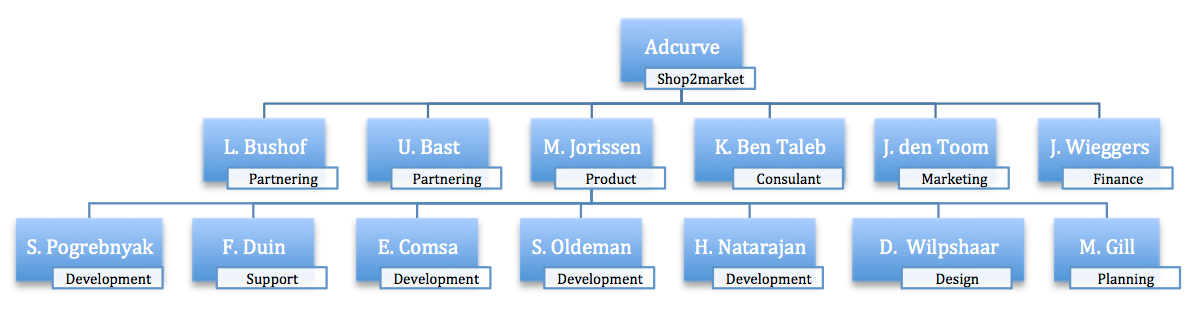
\includegraphics[width=0.9\textwidth]{organisation_structure.png}
    \caption{Organogram waarin het team en de relaties binnen Shop2market worden afgebeeld.}
    \label{fig:orgchart}
\end{figure}


\clearpage

\section{De kwestie} % een kwestie (aanleiding, het op te lossen probleem, de te vervullen behoefte of de te benutten kans);

Zoals te lezen valt in de aanleiding zijn er meerdere redenen voor dit project.

\begin{enumerate}
    \item De tijd die het kost om statistieken te berekenen is aan de hoge kant. De berekeningen worden uitgevoerd met behulp van MongoDB MapReduce. Het team voorziet dat deze technologie niet genoeg schaalbaarheid biedt. Dit omdat rekentijd lineair is toegenomen in relatie tot de hoeveelheid data. Met de verwachte groei van Adcurve komen nieuwe requirements aan het licht en er moet naar een nieuwe oplossing worden gezocht.
    \item Bij voorkeur worden publishers geïntegreerd met behulp van API 's oftewel; een externe data bron. Op deze manier worden berekeningen uitgevoerd met precieze advertentiekosten. Maar doordat externe factoren nu een rol spelen in de berekeningen is het niet te garanderen dat de uitkomst altijd correct is. Zodra fouten intern of extern hersteld zijn, worden berekeningen voor een bepaalde dag, webwinkel of publisher opnieuw uitgevoerd. Het uitvoeren van dit soort correcties is tijdrovend door de huidige implementatie en gebruikte technieken.
    \item Als laatste ontstaat er een kans door de huidige problematiek op te lossen. Webwinkels ontvangen tot soms tot 30 dagen na een bestelling een retournering van een of meerdere producten. Dit betekent dat een product niet verkocht is en de omzet uit de bestelling lager ligt dan is berekend. Het is wenselijk om berekende statistieken met betrekken tot retour bestellingen opnieuw te kunnen berekenen.
\end{enumerate}


\section{Doelstelling} % de doelstellingen (wat moet na afloop van het afstudeerproject zijn bereikt);
\label{sec:doelstelling}

Webwinkel-eigenaren meten in staat zijn om beslissingen te maken op basis van correcte en actuele gegevens in Adcurve. Dit betekent dat de gegevens die Adcurve toont altijd te verklaren zijn en overeenkomen met de werkelijkheid. Daarom moet data op tijd worden verwerkt evenals het tijdig herstellen van fouten mogelijk zijn.

\section{Type opdracht}

Aan de hand van beschikbare technieken wordt er gekozen een aantal mogelijke oplossingen\newline te proberen middels een POC. Dit sluit goed aan bij de aard van een onderzoeksopdracht. Door dit onderzoek moet duidelijk gaan worden: Hoe kan de opdracht worden opgelost? Is dit mogelijk? En wat is er nodig om de oplossing naar productie te krijgen? Door de opdrachtgever is gevraagd om een aantal POC 's te ontwikkelen om tot een inzicht over de oplossing te komen. Er is hierdoor sprake van een ontwikkel opdracht.

